\documentclass[1p]{elsarticle_modified}
%\bibliographystyle{elsarticle-num}

%\usepackage[colorlinks]{hyperref}
%\usepackage{abbrmath_seonhwa} %\Abb, \Ascr, \Acal ,\Abf, \Afrak
\usepackage{amsfonts}
\usepackage{amssymb}
\usepackage{amsmath}
\usepackage{amsthm}
\usepackage{scalefnt}
\usepackage{amsbsy}
\usepackage{kotex}
\usepackage{caption}
\usepackage{subfig}
\usepackage{color}
\usepackage{graphicx}
\usepackage{xcolor} %% white, black, red, green, blue, cyan, magenta, yellow
\usepackage{float}
\usepackage{setspace}
\usepackage{hyperref}

\usepackage{tikz}
\usetikzlibrary{arrows}

\usepackage{multirow}
\usepackage{array} % fixed length table
\usepackage{hhline}

%%%%%%%%%%%%%%%%%%%%%
\makeatletter
\renewcommand*\env@matrix[1][\arraystretch]{%
	\edef\arraystretch{#1}%
	\hskip -\arraycolsep
	\let\@ifnextchar\new@ifnextchar
	\array{*\c@MaxMatrixCols c}}
\makeatother %https://tex.stackexchange.com/questions/14071/how-can-i-increase-the-line-spacing-in-a-matrix
%%%%%%%%%%%%%%%

\usepackage[normalem]{ulem}

\newcommand{\msout}[1]{\ifmmode\text{\sout{\ensuremath{#1}}}\else\sout{#1}\fi}
%SOURCE: \msout is \stkout macro in https://tex.stackexchange.com/questions/20609/strikeout-in-math-mode

\newcommand{\cancel}[1]{
	\ifmmode
	{\color{red}\msout{#1}}
	\else
	{\color{red}\sout{#1}}
	\fi
}

\newcommand{\add}[1]{
	{\color{blue}\uwave{#1}}
}

\newcommand{\replace}[2]{
	\ifmmode
	{\color{red}\msout{#1}}{\color{blue}\uwave{#2}}
	\else
	{\color{red}\sout{#1}}{\color{blue}\uwave{#2}}
	\fi
}

\newcommand{\Sol}{\mathcal{S}} %segment
\newcommand{\D}{D} %diagram
\newcommand{\A}{\mathcal{A}} %arc


%%%%%%%%%%%%%%%%%%%%%%%%%%%%%5 test

\def\sl{\operatorname{\textup{SL}}(2,\Cbb)}
\def\psl{\operatorname{\textup{PSL}}(2,\Cbb)}
\def\quan{\mkern 1mu \triangleright \mkern 1mu}

\theoremstyle{definition}
\newtheorem{thm}{Theorem}[section]
\newtheorem{prop}[thm]{Proposition}
\newtheorem{lem}[thm]{Lemma}
\newtheorem{ques}[thm]{Question}
\newtheorem{cor}[thm]{Corollary}
\newtheorem{defn}[thm]{Definition}
\newtheorem{exam}[thm]{Example}
\newtheorem{rmk}[thm]{Remark}
\newtheorem{alg}[thm]{Algorithm}

\newcommand{\I}{\sqrt{-1}}
\begin{document}

%\begin{frontmatter}
%
%\title{Boundary parabolic representations of knots up to 8 crossings}
%
%%% Group authors per affiliation:
%\author{Yunhi Cho} 
%\address{Department of Mathematics, University of Seoul, Seoul, Korea}
%\ead{yhcho@uos.ac.kr}
%
%
%\author{Seonhwa Kim} %\fnref{s_kim}}
%\address{Center for Geometry and Physics, Institute for Basic Science, Pohang, 37673, Korea}
%\ead{ryeona17@ibs.re.kr}
%
%\author{Hyuk Kim}
%\address{Department of Mathematical Sciences, Seoul National University, Seoul 08826, Korea}
%\ead{hyukkim@snu.ac.kr}
%
%\author{Seokbeom Yoon}
%\address{Department of Mathematical Sciences, Seoul National University, Seoul, 08826,  Korea}
%\ead{sbyoon15@snu.ac.kr}
%
%\begin{abstract}
%We find all boundary parabolic representation of knots up to 8 crossings.
%
%\end{abstract}
%\begin{keyword}
%    \MSC[2010] 57M25 
%\end{keyword}
%
%\end{frontmatter}

%\linenumbers
%\tableofcontents
%
\newcommand\colored[1]{\textcolor{white}{\rule[-0.35ex]{0.8em}{1.4ex}}\kern-0.8em\color{red} #1}%
%\newcommand\colored[1]{\textcolor{white}{ #1}\kern-2.17ex	\textcolor{white}{ #1}\kern-1.81ex	\textcolor{white}{ #1}\kern-2.15ex\color{red}#1	}

{\Large $\underline{12a_{0587}~(K12a_{0587})}$}

\setlength{\tabcolsep}{10pt}
\renewcommand{\arraystretch}{1.6}
\vspace{1cm}\begin{tabular}{m{100pt}>{\centering\arraybackslash}m{274pt}}
\multirow{5}{120pt}{
	\centering
	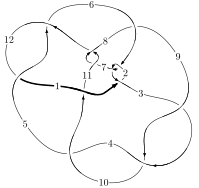
\includegraphics[width=112pt]{../../../GIT/diagram.site/Diagrams/png/1388_12a_0587.png}\\
\ \ \ A knot diagram\footnotemark}&
\allowdisplaybreaks
\textbf{Linearized knot diagam} \\
\cline{2-2}
 &
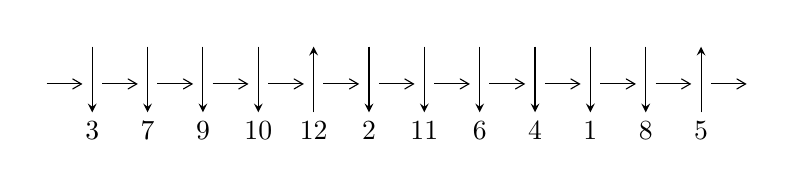
\begin{tikzpicture}[x=20pt, y=17pt]
	% nodes
	\node (C0) at (0, 0) {};
	\node (C1) at (1, 0) {};
	\node (C1U) at (1, +1) {};
	\node (C1D) at (1, -1) {3};

	\node (C2) at (2, 0) {};
	\node (C2U) at (2, +1) {};
	\node (C2D) at (2, -1) {7};

	\node (C3) at (3, 0) {};
	\node (C3U) at (3, +1) {};
	\node (C3D) at (3, -1) {9};

	\node (C4) at (4, 0) {};
	\node (C4U) at (4, +1) {};
	\node (C4D) at (4, -1) {10};

	\node (C5) at (5, 0) {};
	\node (C5U) at (5, +1) {};
	\node (C5D) at (5, -1) {12};

	\node (C6) at (6, 0) {};
	\node (C6U) at (6, +1) {};
	\node (C6D) at (6, -1) {2};

	\node (C7) at (7, 0) {};
	\node (C7U) at (7, +1) {};
	\node (C7D) at (7, -1) {11};

	\node (C8) at (8, 0) {};
	\node (C8U) at (8, +1) {};
	\node (C8D) at (8, -1) {6};

	\node (C9) at (9, 0) {};
	\node (C9U) at (9, +1) {};
	\node (C9D) at (9, -1) {4};

	\node (C10) at (10, 0) {};
	\node (C10U) at (10, +1) {};
	\node (C10D) at (10, -1) {1};

	\node (C11) at (11, 0) {};
	\node (C11U) at (11, +1) {};
	\node (C11D) at (11, -1) {8};

	\node (C12) at (12, 0) {};
	\node (C12U) at (12, +1) {};
	\node (C12D) at (12, -1) {5};
	\node (C13) at (13, 0) {};

	% arrows
	\draw[->,>={angle 60}]
	(C0) edge (C1) (C1) edge (C2) (C2) edge (C3) (C3) edge (C4) (C4) edge (C5) (C5) edge (C6) (C6) edge (C7) (C7) edge (C8) (C8) edge (C9) (C9) edge (C10) (C10) edge (C11) (C11) edge (C12) (C12) edge (C13) ;	\draw[->,>=stealth]
	(C1U) edge (C1D) (C2U) edge (C2D) (C3U) edge (C3D) (C4U) edge (C4D) (C5D) edge (C5U) (C6U) edge (C6D) (C7U) edge (C7D) (C8U) edge (C8D) (C9U) edge (C9D) (C10U) edge (C10D) (C11U) edge (C11D) (C12D) edge (C12U) ;
	\end{tikzpicture} \\
\hhline{~~} \\& 
\textbf{Solving Sequence} \\ \cline{2-2} 
 &
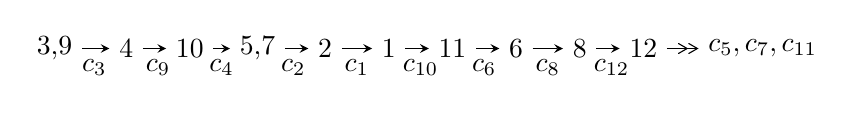
\begin{tikzpicture}[x=23pt, y=7pt]
	% node
	\node (A0) at (-1/8, 0) {3,9};
	\node (A1) at (1, 0) {4};
	\node (A2) at (2, 0) {10};
	\node (A3) at (49/16, 0) {5,7};
	\node (A4) at (33/8, 0) {2};
	\node (A5) at (41/8, 0) {1};
	\node (A6) at (49/8, 0) {11};
	\node (A7) at (57/8, 0) {6};
	\node (A8) at (65/8, 0) {8};
	\node (A9) at (73/8, 0) {12};
	\node (C1) at (1/2, -1) {$c_{3}$};
	\node (C2) at (3/2, -1) {$c_{9}$};
	\node (C3) at (5/2, -1) {$c_{4}$};
	\node (C4) at (29/8, -1) {$c_{2}$};
	\node (C5) at (37/8, -1) {$c_{1}$};
	\node (C6) at (45/8, -1) {$c_{10}$};
	\node (C7) at (53/8, -1) {$c_{6}$};
	\node (C8) at (61/8, -1) {$c_{8}$};
	\node (C9) at (69/8, -1) {$c_{12}$};
	\node (A10) at (11, 0) {$c_{5},c_{7},c_{11}$};

	% edge
	\draw[->,>=stealth]	
	(A0) edge (A1) (A1) edge (A2) (A2) edge (A3) (A3) edge (A4) (A4) edge (A5) (A5) edge (A6) (A6) edge (A7) (A7) edge (A8) (A8) edge (A9) ;
	\draw[->>,>={angle 60}]	
	(A9) edge (A10);
\end{tikzpicture} \\ 

\end{tabular} \\

\footnotetext{
The image of knot diagram is generated by the software ``\textbf{Draw programme}" developed by Andrew Bartholomew(\url{http://www.layer8.co.uk/maths/draw/index.htm\#Running-draw}), where we modified some parts for our purpose(\url{https://github.com/CATsTAILs/LinksPainter}).
}\phantom \\ \newline 
\centering \textbf{Ideals for irreducible components\footnotemark of $X_{\text{par}}$} 
 
\begin{align*}
I^u_{1}&=\langle 
3.83230\times10^{210} u^{94}+2.87938\times10^{210} u^{93}+\cdots+6.01126\times10^{209} b+1.51610\times10^{211},\\
\phantom{I^u_{1}}&\phantom{= \langle  }-6.22396\times10^{212} u^{94}-5.32040\times10^{212} u^{93}+\cdots+1.38259\times10^{211} a-3.59834\times10^{213},\\
\phantom{I^u_{1}}&\phantom{= \langle  }u^{95}+u^{94}+\cdots+14 u+1\rangle \\
I^u_{2}&=\langle 
b+u,\;-5 u^3+u^2+3 a+u+1,\;u^4- u^2+1\rangle \\
I^u_{3}&=\langle 
u^3+b- u,\;-2 u^3-2 u^2+3 a+u+1,\;u^4- u^2+1\rangle \\
\\
\end{align*}
\raggedright * 3 irreducible components of $\dim_{\mathbb{C}}=0$, with total 103 representations.\\
\footnotetext{All coefficients of polynomials are rational numbers. But the coefficients are sometimes approximated in decimal forms when there is not enough margin.}
\newpage
\renewcommand{\arraystretch}{1}
\centering \section*{I. $I^u_{1}= \langle 3.83\times10^{210} u^{94}+2.88\times10^{210} u^{93}+\cdots+6.01\times10^{209} b+1.52\times10^{211},\;-6.22\times10^{212} u^{94}-5.32\times10^{212} u^{93}+\cdots+1.38\times10^{211} a-3.60\times10^{213},\;u^{95}+u^{94}+\cdots+14 u+1 \rangle$}
\flushleft \textbf{(i) Arc colorings}\\
\begin{tabular}{m{7pt} m{180pt} m{7pt} m{180pt} }
\flushright $a_{3}=$&$\begin{pmatrix}1\\0\end{pmatrix}$ \\
\flushright $a_{9}=$&$\begin{pmatrix}0\\u\end{pmatrix}$ \\
\flushright $a_{4}=$&$\begin{pmatrix}1\\u^2\end{pmatrix}$ \\
\flushright $a_{10}=$&$\begin{pmatrix}- u\\- u^3+u\end{pmatrix}$ \\
\flushright $a_{5}=$&$\begin{pmatrix}- u^2+1\\- u^4+2 u^2\end{pmatrix}$ \\
\flushright $a_{7}=$&$\begin{pmatrix}45.0167 u^{94}+38.4814 u^{93}+\cdots+2267.19 u+260.261\\-6.37520 u^{94}-4.78997 u^{93}+\cdots-257.604 u-25.2210\end{pmatrix}$ \\
\flushright $a_{2}=$&$\begin{pmatrix}1.59454 u^{94}+0.308707 u^{93}+\cdots-66.9417 u-32.4693\\7.62210 u^{94}+6.21989 u^{93}+\cdots+361.151 u+39.4626\end{pmatrix}$ \\
\flushright $a_{1}=$&$\begin{pmatrix}9.21664 u^{94}+6.52860 u^{93}+\cdots+294.209 u+6.99328\\7.62210 u^{94}+6.21989 u^{93}+\cdots+361.151 u+39.4626\end{pmatrix}$ \\
\flushright $a_{11}=$&$\begin{pmatrix}-11.7276 u^{94}+0.556507 u^{93}+\cdots+490.732 u+114.762\\-13.6943 u^{94}-10.5472 u^{93}+\cdots-561.915 u-56.4554\end{pmatrix}$ \\
\flushright $a_{6}=$&$\begin{pmatrix}28.2378 u^{94}+25.1088 u^{93}+\cdots+1538.65 u+179.735\\0.930224 u^{94}+1.04484 u^{93}+\cdots+81.7759 u+13.0061\end{pmatrix}$ \\
\flushright $a_{8}=$&$\begin{pmatrix}19.8661 u^{94}+26.6636 u^{93}+\cdots+1975.80 u+268.892\\-12.5392 u^{94}-9.28515 u^{93}+\cdots-487.948 u-46.1105\end{pmatrix}$ \\
\flushright $a_{12}=$&$\begin{pmatrix}3.02163 u^{94}+1.62086 u^{93}+\cdots+14.8334 u-24.3382\\7.07489 u^{94}+5.79666 u^{93}+\cdots+336.703 u+36.8118\end{pmatrix}$\\&\end{tabular}
\flushleft \textbf{(ii) Obstruction class $= -1$}\\~\\
\flushleft \textbf{(iii) Cusp Shapes $= -43.6001 u^{94}-30.2490 u^{93}+\cdots-1486.07 u-149.913$}\\~\\
\newpage\renewcommand{\arraystretch}{1}
\flushleft \textbf{(iv) u-Polynomials at the component}\newline \\
\begin{tabular}{m{50pt}|m{274pt}}
Crossings & \hspace{64pt}u-Polynomials at each crossing \\
\hline $$\begin{aligned}c_{1}\end{aligned}$$&$\begin{aligned}
&u^{95}+45 u^{94}+\cdots+5812 u+169
\end{aligned}$\\
\hline $$\begin{aligned}c_{2},c_{6}\end{aligned}$$&$\begin{aligned}
&u^{95}-3 u^{94}+\cdots-64 u-13
\end{aligned}$\\
\hline $$\begin{aligned}c_{3},c_{4},c_{9}\end{aligned}$$&$\begin{aligned}
&u^{95}- u^{94}+\cdots+14 u-1
\end{aligned}$\\
\hline $$\begin{aligned}c_{5},c_{12}\end{aligned}$$&$\begin{aligned}
&u^{95}-3 u^{94}+\cdots-544 u-52
\end{aligned}$\\
\hline $$\begin{aligned}c_{7},c_{11}\end{aligned}$$&$\begin{aligned}
&u^{95}+5 u^{94}+\cdots-22 u-1
\end{aligned}$\\
\hline $$\begin{aligned}c_{8}\end{aligned}$$&$\begin{aligned}
&529(529 u^{95}-345 u^{94}+\cdots-1.01241\times10^{8} u+1.22522\times10^{7})
\end{aligned}$\\
\hline $$\begin{aligned}c_{10}\end{aligned}$$&$\begin{aligned}
&529(529 u^{95}+1035 u^{94}+\cdots+6.65199\times10^{7} u+1.26008\times10^{7})
\end{aligned}$\\
\hline
\end{tabular}\\~\\
\newpage\renewcommand{\arraystretch}{1}
\flushleft \textbf{(v) Riley Polynomials at the component}\newline \\
\begin{tabular}{m{50pt}|m{274pt}}
Crossings & \hspace{64pt}Riley Polynomials at each crossing \\
\hline $$\begin{aligned}c_{1}\end{aligned}$$&$\begin{aligned}
&y^{95}+15 y^{94}+\cdots+2924000 y-28561
\end{aligned}$\\
\hline $$\begin{aligned}c_{2},c_{6}\end{aligned}$$&$\begin{aligned}
&y^{95}-45 y^{94}+\cdots+5812 y-169
\end{aligned}$\\
\hline $$\begin{aligned}c_{3},c_{4},c_{9}\end{aligned}$$&$\begin{aligned}
&y^{95}-93 y^{94}+\cdots+88 y-1
\end{aligned}$\\
\hline $$\begin{aligned}c_{5},c_{12}\end{aligned}$$&$\begin{aligned}
&y^{95}+83 y^{94}+\cdots-1192 y-2704
\end{aligned}$\\
\hline $$\begin{aligned}c_{7},c_{11}\end{aligned}$$&$\begin{aligned}
&y^{95}-57 y^{94}+\cdots+304 y-1
\end{aligned}$\\
\hline $$\begin{aligned}c_{8}\end{aligned}$$&$\begin{aligned}
&279841(279841 y^{95}-2.19233\times10^{7} y^{94}+\cdots+8.54386\times10^{15} y-1.50117\times10^{14})
\end{aligned}$\\
\hline $$\begin{aligned}c_{10}\end{aligned}$$&$\begin{aligned}
&279841(279841 y^{95}-1.00515\times10^{7} y^{94}+\cdots+2.52702\times10^{16} y-1.58780\times10^{14})
\end{aligned}$\\
\hline
\end{tabular}\\~\\
\newpage\flushleft \textbf{(vi) Complex Volumes and Cusp Shapes}
$$\begin{array}{c|c|c}  
\text{Solutions to }I^u_{1}& \I (\text{vol} + \sqrt{-1}CS) & \text{Cusp shape}\\
 \hline 
\begin{aligned}
u &= \phantom{-}0.324076 + 0.932614 I \\
a &= -0.57215 - 1.46473 I \\
b &= \phantom{-}1.106370 + 0.298292 I\end{aligned}
 & -8.62975 - 0.07531 I & \phantom{-0.000000 } 0 \\ \hline\begin{aligned}
u &= \phantom{-}0.324076 - 0.932614 I \\
a &= -0.57215 + 1.46473 I \\
b &= \phantom{-}1.106370 - 0.298292 I\end{aligned}
 & -8.62975 + 0.07531 I & \phantom{-0.000000 } 0 \\ \hline\begin{aligned}
u &= \phantom{-}0.740982 + 0.622306 I \\
a &= \phantom{-}0.271489 + 0.025604 I \\
b &= -1.207240 + 0.119440 I\end{aligned}
 & -10.13730 - 5.06463 I & \phantom{-0.000000 } 0 \\ \hline\begin{aligned}
u &= \phantom{-}0.740982 - 0.622306 I \\
a &= \phantom{-}0.271489 - 0.025604 I \\
b &= -1.207240 - 0.119440 I\end{aligned}
 & -10.13730 + 5.06463 I & \phantom{-0.000000 } 0 \\ \hline\begin{aligned}
u &= \phantom{-}0.893227 + 0.368349 I \\
a &= -0.219033 + 0.457967 I \\
b &= \phantom{-}0.831308 - 0.551679 I\end{aligned}
 & -0.1180870 + 0.0250280 I & \phantom{-0.000000 } 0 \\ \hline\begin{aligned}
u &= \phantom{-}0.893227 - 0.368349 I \\
a &= -0.219033 - 0.457967 I \\
b &= \phantom{-}0.831308 + 0.551679 I\end{aligned}
 & -0.1180870 - 0.0250280 I & \phantom{-0.000000 } 0 \\ \hline\begin{aligned}
u &= \phantom{-}0.569885 + 0.872471 I \\
a &= -0.19005 - 1.86439 I \\
b &= \phantom{-}1.143560 + 0.616829 I\end{aligned}
 & -6.8689 - 13.3214 I & \phantom{-0.000000 } 0 \\ \hline\begin{aligned}
u &= \phantom{-}0.569885 - 0.872471 I \\
a &= -0.19005 + 1.86439 I \\
b &= \phantom{-}1.143560 - 0.616829 I\end{aligned}
 & -6.8689 + 13.3214 I & \phantom{-0.000000 } 0 \\ \hline\begin{aligned}
u &= -0.530173 + 0.768074 I \\
a &= -0.75856 - 1.22838 I \\
b &= \phantom{-}0.385983 + 0.866786 I\end{aligned}
 & -4.58095 + 7.84168 I & \phantom{-0.000000 } 0 \\ \hline\begin{aligned}
u &= -0.530173 - 0.768074 I \\
a &= -0.75856 + 1.22838 I \\
b &= \phantom{-}0.385983 - 0.866786 I\end{aligned}
 & -4.58095 - 7.84168 I & \phantom{-0.000000 } 0\\
 \hline 
 \end{array}$$\newpage$$\begin{array}{c|c|c}  
\text{Solutions to }I^u_{1}& \I (\text{vol} + \sqrt{-1}CS) & \text{Cusp shape}\\
 \hline 
\begin{aligned}
u &= -0.563129 + 0.738059 I \\
a &= -0.28918 - 1.51880 I \\
b &= -0.284444 + 0.674957 I\end{aligned}
 & -4.69329 - 2.77756 I & \phantom{-0.000000 } 0 \\ \hline\begin{aligned}
u &= -0.563129 - 0.738059 I \\
a &= -0.28918 + 1.51880 I \\
b &= -0.284444 - 0.674957 I\end{aligned}
 & -4.69329 + 2.77756 I & \phantom{-0.000000 } 0 \\ \hline\begin{aligned}
u &= \phantom{-}0.461536 + 0.798582 I \\
a &= -0.528916 + 1.097220 I \\
b &= \phantom{-}0.413376 - 0.527923 I\end{aligned}
 & -0.62347 - 2.22932 I & \phantom{-0.000000 } 0 \\ \hline\begin{aligned}
u &= \phantom{-}0.461536 - 0.798582 I \\
a &= -0.528916 - 1.097220 I \\
b &= \phantom{-}0.413376 + 0.527923 I\end{aligned}
 & -0.62347 + 2.22932 I & \phantom{-0.000000 } 0 \\ \hline\begin{aligned}
u &= -1.028620 + 0.372700 I \\
a &= \phantom{-}0.336932 + 1.297890 I \\
b &= \phantom{-}0.792047 - 0.591034 I\end{aligned}
 & \phantom{-}0.00681 + 4.54787 I & \phantom{-0.000000 } 0 \\ \hline\begin{aligned}
u &= -1.028620 - 0.372700 I \\
a &= \phantom{-}0.336932 - 1.297890 I \\
b &= \phantom{-}0.792047 + 0.591034 I\end{aligned}
 & \phantom{-}0.00681 - 4.54787 I & \phantom{-0.000000 } 0 \\ \hline\begin{aligned}
u &= \phantom{-}0.657206 + 0.901845 I \\
a &= \phantom{-}0.644915 - 0.664953 I \\
b &= -1.111150 + 0.535210 I\end{aligned}
 & -7.03870 + 7.43919 I & \phantom{-0.000000 } 0 \\ \hline\begin{aligned}
u &= \phantom{-}0.657206 - 0.901845 I \\
a &= \phantom{-}0.644915 + 0.664953 I \\
b &= -1.111150 - 0.535210 I\end{aligned}
 & -7.03870 - 7.43919 I & \phantom{-0.000000 } 0 \\ \hline\begin{aligned}
u &= -0.555423 + 1.010360 I \\
a &= -0.23176 + 1.60411 I \\
b &= \phantom{-}1.060760 - 0.514305 I\end{aligned}
 & -2.49114 + 6.53115 I & \phantom{-0.000000 } 0 \\ \hline\begin{aligned}
u &= -0.555423 - 1.010360 I \\
a &= -0.23176 - 1.60411 I \\
b &= \phantom{-}1.060760 + 0.514305 I\end{aligned}
 & -2.49114 - 6.53115 I & \phantom{-0.000000 } 0\\
 \hline 
 \end{array}$$\newpage$$\begin{array}{c|c|c}  
\text{Solutions to }I^u_{1}& \I (\text{vol} + \sqrt{-1}CS) & \text{Cusp shape}\\
 \hline 
\begin{aligned}
u &= -0.445712 + 0.635397 I \\
a &= \phantom{-}0.11193 - 1.81470 I \\
b &= -1.139330 + 0.600773 I\end{aligned}
 & -1.72270 + 8.42111 I & \phantom{-0.000000 } 0 \\ \hline\begin{aligned}
u &= -0.445712 - 0.635397 I \\
a &= \phantom{-}0.11193 + 1.81470 I \\
b &= -1.139330 - 0.600773 I\end{aligned}
 & -1.72270 - 8.42111 I & \phantom{-0.000000 } 0 \\ \hline\begin{aligned}
u &= \phantom{-}1.066390 + 0.614208 I \\
a &= -0.16248 + 1.40511 I \\
b &= -0.778605 - 0.254375 I\end{aligned}
 & -2.29481 - 2.77237 I & \phantom{-0.000000 } 0 \\ \hline\begin{aligned}
u &= \phantom{-}1.066390 - 0.614208 I \\
a &= -0.16248 - 1.40511 I \\
b &= -0.778605 + 0.254375 I\end{aligned}
 & -2.29481 + 2.77237 I & \phantom{-0.000000 } 0 \\ \hline\begin{aligned}
u &= -0.890509 + 0.889227 I \\
a &= \phantom{-}0.352038 + 0.577350 I \\
b &= -1.021720 - 0.391174 I\end{aligned}
 & -3.42941 - 0.01024 I & \phantom{-0.000000 } 0 \\ \hline\begin{aligned}
u &= -0.890509 - 0.889227 I \\
a &= \phantom{-}0.352038 - 0.577350 I \\
b &= -1.021720 + 0.391174 I\end{aligned}
 & -3.42941 + 0.01024 I & \phantom{-0.000000 } 0 \\ \hline\begin{aligned}
u &= \phantom{-}0.337463 + 0.657456 I \\
a &= \phantom{-}0.20569 + 2.01133 I \\
b &= -0.979429 - 0.576485 I\end{aligned}
 & \phantom{-}1.42526 - 3.92148 I & \phantom{-0.000000 } 0 \\ \hline\begin{aligned}
u &= \phantom{-}0.337463 - 0.657456 I \\
a &= \phantom{-}0.20569 - 2.01133 I \\
b &= -0.979429 + 0.576485 I\end{aligned}
 & \phantom{-}1.42526 + 3.92148 I & \phantom{-0.000000 } 0 \\ \hline\begin{aligned}
u &= -0.519994 + 0.514146 I \\
a &= -0.573261 + 0.194172 I \\
b &= \phantom{-}1.027730 + 0.525528 I\end{aligned}
 & -2.04737 - 4.42997 I & \phantom{-0.000000 } 0 \\ \hline\begin{aligned}
u &= -0.519994 - 0.514146 I \\
a &= -0.573261 - 0.194172 I \\
b &= \phantom{-}1.027730 - 0.525528 I\end{aligned}
 & -2.04737 + 4.42997 I & \phantom{-0.000000 } 0\\
 \hline 
 \end{array}$$\newpage$$\begin{array}{c|c|c}  
\text{Solutions to }I^u_{1}& \I (\text{vol} + \sqrt{-1}CS) & \text{Cusp shape}\\
 \hline 
\begin{aligned}
u &= -0.688347 + 0.015904 I \\
a &= -1.00082 - 1.58321 I \\
b &= -0.745151 - 0.178389 I\end{aligned}
 & -3.31796 - 2.34016 I & -17.3652 + 3.7071 I \\ \hline\begin{aligned}
u &= -0.688347 - 0.015904 I \\
a &= -1.00082 + 1.58321 I \\
b &= -0.745151 + 0.178389 I\end{aligned}
 & -3.31796 + 2.34016 I & -17.3652 - 3.7071 I \\ \hline\begin{aligned}
u &= \phantom{-}0.634046 + 0.217215 I \\
a &= \phantom{-}0.789475 - 0.701622 I \\
b &= \phantom{-}0.546456 + 0.509073 I\end{aligned}
 & -0.559909 + 0.111371 I & -8.00000 + 1.58099 I \\ \hline\begin{aligned}
u &= \phantom{-}0.634046 - 0.217215 I \\
a &= \phantom{-}0.789475 + 0.701622 I \\
b &= \phantom{-}0.546456 - 0.509073 I\end{aligned}
 & -0.559909 - 0.111371 I & -8.00000 - 1.58099 I \\ \hline\begin{aligned}
u &= -0.167463 + 0.634472 I \\
a &= \phantom{-}0.94089 + 1.19979 I \\
b &= -0.616501 - 0.643520 I\end{aligned}
 & \phantom{-}2.51116 - 0.85388 I & -1.53097 + 2.15494 I \\ \hline\begin{aligned}
u &= -0.167463 - 0.634472 I \\
a &= \phantom{-}0.94089 - 1.19979 I \\
b &= -0.616501 + 0.643520 I\end{aligned}
 & \phantom{-}2.51116 + 0.85388 I & -1.53097 - 2.15494 I \\ \hline\begin{aligned}
u &= -1.349460 + 0.003354 I \\
a &= -1.023390 - 0.016086 I \\
b &= \phantom{-}0.363060 + 0.020561 I\end{aligned}
 & -6.49407 + 0.00002 I & \phantom{-0.000000 } 0 \\ \hline\begin{aligned}
u &= -1.349460 - 0.003354 I \\
a &= -1.023390 + 0.016086 I \\
b &= \phantom{-}0.363060 - 0.020561 I\end{aligned}
 & -6.49407 - 0.00002 I & \phantom{-0.000000 } 0 \\ \hline\begin{aligned}
u &= \phantom{-}1.370850 + 0.152453 I \\
a &= -0.394075 + 0.330422 I \\
b &= \phantom{-}0.391587 - 0.786955 I\end{aligned}
 & -2.29932 - 1.84849 I & \phantom{-0.000000 } 0 \\ \hline\begin{aligned}
u &= \phantom{-}1.370850 - 0.152453 I \\
a &= -0.394075 - 0.330422 I \\
b &= \phantom{-}0.391587 + 0.786955 I\end{aligned}
 & -2.29932 + 1.84849 I & \phantom{-0.000000 } 0\\
 \hline 
 \end{array}$$\newpage$$\begin{array}{c|c|c}  
\text{Solutions to }I^u_{1}& \I (\text{vol} + \sqrt{-1}CS) & \text{Cusp shape}\\
 \hline 
\begin{aligned}
u &= \phantom{-}0.285873 + 0.537667 I \\
a &= \phantom{-}0.640866 - 1.135400 I \\
b &= -0.334758 + 0.847402 I\end{aligned}
 & \phantom{-}0.65285 - 3.08282 I & -5.72735 + 6.58681 I \\ \hline\begin{aligned}
u &= \phantom{-}0.285873 - 0.537667 I \\
a &= \phantom{-}0.640866 + 1.135400 I \\
b &= -0.334758 - 0.847402 I\end{aligned}
 & \phantom{-}0.65285 + 3.08282 I & -5.72735 - 6.58681 I \\ \hline\begin{aligned}
u &= -1.41992 + 0.06769 I \\
a &= \phantom{-}0.423092 - 0.516069 I \\
b &= -0.578569 + 0.777127 I\end{aligned}
 & -5.89719 + 3.01762 I & \phantom{-0.000000 } 0 \\ \hline\begin{aligned}
u &= -1.41992 - 0.06769 I \\
a &= \phantom{-}0.423092 + 0.516069 I \\
b &= -0.578569 - 0.777127 I\end{aligned}
 & -5.89719 - 3.01762 I & \phantom{-0.000000 } 0 \\ \hline\begin{aligned}
u &= -1.42403 + 0.14320 I \\
a &= -0.293544 - 0.361005 I \\
b &= \phantom{-}0.199462 + 1.104120 I\end{aligned}
 & -4.83461 + 5.45013 I & \phantom{-0.000000 } 0 \\ \hline\begin{aligned}
u &= -1.42403 - 0.14320 I \\
a &= -0.293544 + 0.361005 I \\
b &= \phantom{-}0.199462 - 1.104120 I\end{aligned}
 & -4.83461 - 5.45013 I & \phantom{-0.000000 } 0 \\ \hline\begin{aligned}
u &= \phantom{-}1.42892 + 0.08720 I \\
a &= -0.92447 + 1.27995 I \\
b &= -0.961852 + 0.399126 I\end{aligned}
 & -8.27189 + 2.49117 I & \phantom{-0.000000 } 0 \\ \hline\begin{aligned}
u &= \phantom{-}1.42892 - 0.08720 I \\
a &= -0.92447 - 1.27995 I \\
b &= -0.961852 - 0.399126 I\end{aligned}
 & -8.27189 - 2.49117 I & \phantom{-0.000000 } 0 \\ \hline\begin{aligned}
u &= \phantom{-}1.43420 + 0.13326 I \\
a &= \phantom{-}1.52406 - 1.83104 I \\
b &= \phantom{-}1.017390 + 0.428965 I\end{aligned}
 & -8.23402 - 3.27950 I & \phantom{-0.000000 } 0 \\ \hline\begin{aligned}
u &= \phantom{-}1.43420 - 0.13326 I \\
a &= \phantom{-}1.52406 + 1.83104 I \\
b &= \phantom{-}1.017390 - 0.428965 I\end{aligned}
 & -8.23402 + 3.27950 I & \phantom{-0.000000 } 0\\
 \hline 
 \end{array}$$\newpage$$\begin{array}{c|c|c}  
\text{Solutions to }I^u_{1}& \I (\text{vol} + \sqrt{-1}CS) & \text{Cusp shape}\\
 \hline 
\begin{aligned}
u &= \phantom{-}1.45321 + 0.01462 I \\
a &= -1.08757 + 1.42578 I \\
b &= -1.042040 - 0.600114 I\end{aligned}
 & -7.36301 - 2.23164 I & \phantom{-0.000000 } 0 \\ \hline\begin{aligned}
u &= \phantom{-}1.45321 - 0.01462 I \\
a &= -1.08757 - 1.42578 I \\
b &= -1.042040 + 0.600114 I\end{aligned}
 & -7.36301 + 2.23164 I & \phantom{-0.000000 } 0 \\ \hline\begin{aligned}
u &= \phantom{-}1.45978 + 0.07323 I \\
a &= -0.090635 + 0.736569 I \\
b &= -0.77265 - 1.19938 I\end{aligned}
 & -8.95103 - 5.08029 I & \phantom{-0.000000 } 0 \\ \hline\begin{aligned}
u &= \phantom{-}1.45978 - 0.07323 I \\
a &= -0.090635 - 0.736569 I \\
b &= -0.77265 + 1.19938 I\end{aligned}
 & -8.95103 + 5.08029 I & \phantom{-0.000000 } 0 \\ \hline\begin{aligned}
u &= -1.45946 + 0.20650 I \\
a &= \phantom{-}0.89169 + 1.37027 I \\
b &= \phantom{-}1.106580 - 0.585561 I\end{aligned}
 & -4.42188 + 6.98601 I & \phantom{-0.000000 } 0 \\ \hline\begin{aligned}
u &= -1.45946 - 0.20650 I \\
a &= \phantom{-}0.89169 - 1.37027 I \\
b &= \phantom{-}1.106580 + 0.585561 I\end{aligned}
 & -4.42188 - 6.98601 I & \phantom{-0.000000 } 0 \\ \hline\begin{aligned}
u &= -1.48216 + 0.02984 I \\
a &= -0.467979 - 0.695967 I \\
b &= -1.42038 + 0.80271 I\end{aligned}
 & -11.08730 + 2.97745 I & \phantom{-0.000000 } 0 \\ \hline\begin{aligned}
u &= -1.48216 - 0.02984 I \\
a &= -0.467979 + 0.695967 I \\
b &= -1.42038 - 0.80271 I\end{aligned}
 & -11.08730 - 2.97745 I & \phantom{-0.000000 } 0 \\ \hline\begin{aligned}
u &= -1.48776 + 0.00307 I \\
a &= -1.174830 + 0.041396 I \\
b &= -0.948018 - 0.139900 I\end{aligned}
 & -7.28570 - 0.05797 I & \phantom{-0.000000 } 0 \\ \hline\begin{aligned}
u &= -1.48776 - 0.00307 I \\
a &= -1.174830 - 0.041396 I \\
b &= -0.948018 + 0.139900 I\end{aligned}
 & -7.28570 + 0.05797 I & \phantom{-0.000000 } 0\\
 \hline 
 \end{array}$$\newpage$$\begin{array}{c|c|c}  
\text{Solutions to }I^u_{1}& \I (\text{vol} + \sqrt{-1}CS) & \text{Cusp shape}\\
 \hline 
\begin{aligned}
u &= -0.512086\phantom{ +0.000000I} \\
a &= -0.351550\phantom{ +0.000000I} \\
b &= \phantom{-}1.26425\phantom{ +0.000000I}\end{aligned}
 & -5.16409\phantom{ +0.000000I} & -21.4310\phantom{ +0.000000I} \\ \hline\begin{aligned}
u &= \phantom{-}1.49274\phantom{ +0.000000I} \\
a &= -0.625686\phantom{ +0.000000I} \\
b &= -1.62427\phantom{ +0.000000I}\end{aligned}
 & -11.6983\phantom{ +0.000000I} & \phantom{-0.000000 } 0 \\ \hline\begin{aligned}
u &= \phantom{-}0.234531 + 0.448531 I \\
a &= -0.597145 + 0.065732 I \\
b &= \phantom{-}0.369329 + 0.395606 I\end{aligned}
 & -0.71598 - 1.49940 I & -6.15907 + 3.34895 I \\ \hline\begin{aligned}
u &= \phantom{-}0.234531 - 0.448531 I \\
a &= -0.597145 - 0.065732 I \\
b &= \phantom{-}0.369329 - 0.395606 I\end{aligned}
 & -0.71598 + 1.49940 I & -6.15907 - 3.34895 I \\ \hline\begin{aligned}
u &= \phantom{-}1.49156 + 0.20895 I \\
a &= \phantom{-}0.83745 - 1.19974 I \\
b &= \phantom{-}1.250940 + 0.625768 I\end{aligned}
 & -8.04831 - 11.47770 I & \phantom{-0.000000 } 0 \\ \hline\begin{aligned}
u &= \phantom{-}1.49156 - 0.20895 I \\
a &= \phantom{-}0.83745 + 1.19974 I \\
b &= \phantom{-}1.250940 - 0.625768 I\end{aligned}
 & -8.04831 + 11.47770 I & \phantom{-0.000000 } 0 \\ \hline\begin{aligned}
u &= -0.337519 + 0.313167 I \\
a &= -0.81445 + 1.60127 I \\
b &= \phantom{-}0.643763 - 0.919367 I\end{aligned}
 & -3.06247 + 3.79289 I & -12.8027 - 12.4163 I \\ \hline\begin{aligned}
u &= -0.337519 - 0.313167 I \\
a &= -0.81445 - 1.60127 I \\
b &= \phantom{-}0.643763 + 0.919367 I\end{aligned}
 & -3.06247 - 3.79289 I & -12.8027 + 12.4163 I \\ \hline\begin{aligned}
u &= \phantom{-}0.457671\phantom{ +0.000000I} \\
a &= \phantom{-}0.744423\phantom{ +0.000000I} \\
b &= \phantom{-}0.436249\phantom{ +0.000000I}\end{aligned}
 & -0.800628\phantom{ +0.000000I} & -11.8890\phantom{ +0.000000I} \\ \hline\begin{aligned}
u &= \phantom{-}1.52280 + 0.25579 I \\
a &= \phantom{-}0.446441 - 0.808912 I \\
b &= -0.057837 + 0.708672 I\end{aligned}
 & -11.46720 - 0.79382 I & \phantom{-0.000000 } 0\\
 \hline 
 \end{array}$$\newpage$$\begin{array}{c|c|c}  
\text{Solutions to }I^u_{1}& \I (\text{vol} + \sqrt{-1}CS) & \text{Cusp shape}\\
 \hline 
\begin{aligned}
u &= \phantom{-}1.52280 - 0.25579 I \\
a &= \phantom{-}0.446441 + 0.808912 I \\
b &= -0.057837 - 0.708672 I\end{aligned}
 & -11.46720 + 0.79382 I & \phantom{-0.000000 } 0 \\ \hline\begin{aligned}
u &= -1.53199 + 0.27313 I \\
a &= \phantom{-}0.435468 + 0.585455 I \\
b &= -0.366714 - 0.819444 I\end{aligned}
 & -7.20531 + 6.12991 I & \phantom{-0.000000 } 0 \\ \hline\begin{aligned}
u &= -1.53199 - 0.27313 I \\
a &= \phantom{-}0.435468 - 0.585455 I \\
b &= -0.366714 + 0.819444 I\end{aligned}
 & -7.20531 - 6.12991 I & \phantom{-0.000000 } 0 \\ \hline\begin{aligned}
u &= -0.089043 + 0.433089 I \\
a &= \phantom{-}2.65903 - 3.82631 I \\
b &= -0.952211 + 0.388329 I\end{aligned}
 & -3.11696 + 1.47900 I & -4.54348 - 4.47757 I \\ \hline\begin{aligned}
u &= -0.089043 - 0.433089 I \\
a &= \phantom{-}2.65903 + 3.82631 I \\
b &= -0.952211 - 0.388329 I\end{aligned}
 & -3.11696 - 1.47900 I & -4.54348 + 4.47757 I \\ \hline\begin{aligned}
u &= \phantom{-}1.53594 + 0.26544 I \\
a &= \phantom{-}0.568714 - 0.525422 I \\
b &= -0.387652 + 0.998965 I\end{aligned}
 & -11.3324 - 11.6288 I & \phantom{-0.000000 } 0 \\ \hline\begin{aligned}
u &= \phantom{-}1.53594 - 0.26544 I \\
a &= \phantom{-}0.568714 + 0.525422 I \\
b &= -0.387652 - 0.998965 I\end{aligned}
 & -11.3324 + 11.6288 I & \phantom{-0.000000 } 0 \\ \hline\begin{aligned}
u &= \phantom{-}0.422131 + 0.107983 I \\
a &= -0.45738 - 1.67606 I \\
b &= \phantom{-}1.171970 + 0.672778 I\end{aligned}
 & -4.81368 - 2.48540 I & -22.8854 + 6.6337 I \\ \hline\begin{aligned}
u &= \phantom{-}0.422131 - 0.107983 I \\
a &= -0.45738 + 1.67606 I \\
b &= \phantom{-}1.171970 - 0.672778 I\end{aligned}
 & -4.81368 + 2.48540 I & -22.8854 - 6.6337 I \\ \hline\begin{aligned}
u &= -1.53098 + 0.39379 I \\
a &= -0.40652 - 1.44972 I \\
b &= -1.151730 + 0.452179 I\end{aligned}
 & -14.5947 + 5.0254 I & \phantom{-0.000000 } 0\\
 \hline 
 \end{array}$$\newpage$$\begin{array}{c|c|c}  
\text{Solutions to }I^u_{1}& \I (\text{vol} + \sqrt{-1}CS) & \text{Cusp shape}\\
 \hline 
\begin{aligned}
u &= -1.53098 - 0.39379 I \\
a &= -0.40652 + 1.44972 I \\
b &= -1.151730 - 0.452179 I\end{aligned}
 & -14.5947 - 5.0254 I & \phantom{-0.000000 } 0 \\ \hline\begin{aligned}
u &= -1.57837 + 0.18063 I \\
a &= \phantom{-}0.587660 + 0.219510 I \\
b &= \phantom{-}1.386840 + 0.091526 I\end{aligned}
 & -17.8165 + 7.9839 I & \phantom{-0.000000 } 0 \\ \hline\begin{aligned}
u &= -1.57837 - 0.18063 I \\
a &= \phantom{-}0.587660 - 0.219510 I \\
b &= \phantom{-}1.386840 - 0.091526 I\end{aligned}
 & -17.8165 - 7.9839 I & \phantom{-0.000000 } 0 \\ \hline\begin{aligned}
u &= -1.56353 + 0.30289 I \\
a &= -0.67347 - 1.52002 I \\
b &= -1.192820 + 0.662030 I\end{aligned}
 & -13.8217 + 17.6321 I & \phantom{-0.000000 } 0 \\ \hline\begin{aligned}
u &= -1.56353 - 0.30289 I \\
a &= -0.67347 + 1.52002 I \\
b &= -1.192820 - 0.662030 I\end{aligned}
 & -13.8217 - 17.6321 I & \phantom{-0.000000 } 0 \\ \hline\begin{aligned}
u &= \phantom{-}1.58570 + 0.33378 I \\
a &= -0.58741 + 1.42117 I \\
b &= -1.134900 - 0.594549 I\end{aligned}
 & -9.5017 - 11.4013 I & \phantom{-0.000000 } 0 \\ \hline\begin{aligned}
u &= \phantom{-}1.58570 - 0.33378 I \\
a &= -0.58741 - 1.42117 I \\
b &= -1.134900 + 0.594549 I\end{aligned}
 & -9.5017 + 11.4013 I & \phantom{-0.000000 } 0 \\ \hline\begin{aligned}
u &= \phantom{-}1.62550 + 0.15463 I \\
a &= \phantom{-}0.672705 + 0.179863 I \\
b &= \phantom{-}1.158440 - 0.175281 I\end{aligned}
 & -12.26950 - 3.43058 I & \phantom{-0.000000 } 0 \\ \hline\begin{aligned}
u &= \phantom{-}1.62550 - 0.15463 I \\
a &= \phantom{-}0.672705 - 0.179863 I \\
b &= \phantom{-}1.158440 + 0.175281 I\end{aligned}
 & -12.26950 + 3.43058 I & \phantom{-0.000000 } 0 \\ \hline\begin{aligned}
u &= -1.66015 + 0.23571 I \\
a &= \phantom{-}0.309280 - 0.288553 I \\
b &= \phantom{-}1.152050 + 0.402083 I\end{aligned}
 & -14.9337 - 3.0765 I & \phantom{-0.000000 } 0\\
 \hline 
 \end{array}$$\newpage$$\begin{array}{c|c|c}  
\text{Solutions to }I^u_{1}& \I (\text{vol} + \sqrt{-1}CS) & \text{Cusp shape}\\
 \hline 
\begin{aligned}
u &= -1.66015 - 0.23571 I \\
a &= \phantom{-}0.309280 + 0.288553 I \\
b &= \phantom{-}1.152050 - 0.402083 I\end{aligned}
 & -14.9337 + 3.0765 I & \phantom{-0.000000 } 0 \\ \hline\begin{aligned}
u &= -0.254207 + 0.093976 I \\
a &= -0.02448 - 12.67700 I \\
b &= -0.775297 - 0.496292 I\end{aligned}
 & -3.15119 - 2.08241 I & -30.9227 - 13.8100 I \\ \hline\begin{aligned}
u &= -0.254207 - 0.093976 I \\
a &= -0.02448 + 12.67700 I \\
b &= -0.775297 + 0.496292 I\end{aligned}
 & -3.15119 + 2.08241 I & -30.9227 + 13.8100 I \\ \hline\begin{aligned}
u &= -0.197015 + 0.025110 I \\
a &= \phantom{-}2.85799 + 5.76242 I \\
b &= \phantom{-}0.903883 - 0.528559 I\end{aligned}
 & -1.74590 + 2.04516 I & -12.58558 - 2.81237 I \\ \hline\begin{aligned}
u &= -0.197015 - 0.025110 I \\
a &= \phantom{-}2.85799 - 5.76242 I \\
b &= \phantom{-}0.903883 + 0.528559 I\end{aligned}
 & -1.74590 - 2.04516 I & -12.58558 + 2.81237 I\\
 \hline 
 \end{array}$$\newpage\newpage\renewcommand{\arraystretch}{1}
\centering \section*{II. $I^u_{2}= \langle b+u,\;-5 u^3+u^2+3 a+u+1,\;u^4- u^2+1 \rangle$}
\flushleft \textbf{(i) Arc colorings}\\
\begin{tabular}{m{7pt} m{180pt} m{7pt} m{180pt} }
\flushright $a_{3}=$&$\begin{pmatrix}1\\0\end{pmatrix}$ \\
\flushright $a_{9}=$&$\begin{pmatrix}0\\u\end{pmatrix}$ \\
\flushright $a_{4}=$&$\begin{pmatrix}1\\u^2\end{pmatrix}$ \\
\flushright $a_{10}=$&$\begin{pmatrix}- u\\- u^3+u\end{pmatrix}$ \\
\flushright $a_{5}=$&$\begin{pmatrix}- u^2+1\\u^2+1\end{pmatrix}$ \\
\flushright $a_{7}=$&$\begin{pmatrix}\frac{5}{3} u^3-\frac{1}{3} u^2-\frac{1}{3} u-\frac{1}{3}\\- u\end{pmatrix}$ \\
\flushright $a_{2}=$&$\begin{pmatrix}-\frac{1}{3} u^3+\frac{4}{3} u^2-\frac{1}{3} u-\frac{2}{3}\\- u^2\end{pmatrix}$ \\
\flushright $a_{1}=$&$\begin{pmatrix}-\frac{1}{3} u^3+\frac{1}{3} u^2-\frac{1}{3} u-\frac{2}{3}\\- u^2\end{pmatrix}$ \\
\flushright $a_{11}=$&$\begin{pmatrix}-\frac{1}{3} u^3-\frac{1}{3} u^2-\frac{4}{3} u\\-\frac{5}{3} u^3-\frac{2}{3} u^2+\frac{4}{3} u+\frac{1}{3}\end{pmatrix}$ \\
\flushright $a_{6}=$&$\begin{pmatrix}\frac{1}{3} u^3+\frac{1}{3} u^2+\frac{1}{3} u-\frac{2}{3}\\u^3- u\end{pmatrix}$ \\
\flushright $a_{8}=$&$\begin{pmatrix}-\frac{2}{3} u^2\\-\frac{1}{3} u^3-\frac{1}{3} u^2+\frac{2}{3} u+\frac{2}{3}\end{pmatrix}$ \\
\flushright $a_{12}=$&$\begin{pmatrix}-\frac{1}{3} u^3+\frac{1}{3} u^2-\frac{4}{3} u-\frac{2}{3}\\-2 u^3- u^2+u\end{pmatrix}$\\&\end{tabular}
\flushleft \textbf{(ii) Obstruction class $= 1$}\\~\\
\flushleft \textbf{(iii) Cusp Shapes $= 8 u^2-16$}\\~\\
\newpage\renewcommand{\arraystretch}{1}
\flushleft \textbf{(iv) u-Polynomials at the component}\newline \\
\begin{tabular}{m{50pt}|m{274pt}}
Crossings & \hspace{64pt}u-Polynomials at each crossing \\
\hline $$\begin{aligned}c_{1},c_{7}\end{aligned}$$&$\begin{aligned}
&(u^2- u+1)^2
\end{aligned}$\\
\hline $$\begin{aligned}c_{2},c_{3},c_{4}\\c_{6},c_{9}\end{aligned}$$&$\begin{aligned}
&u^4- u^2+1
\end{aligned}$\\
\hline $$\begin{aligned}c_{5},c_{12}\end{aligned}$$&$\begin{aligned}
&(u^2+1)^2
\end{aligned}$\\
\hline $$\begin{aligned}c_{8}\end{aligned}$$&$\begin{aligned}
&9(9 u^4+4)
\end{aligned}$\\
\hline $$\begin{aligned}c_{10}\end{aligned}$$&$\begin{aligned}
&9(9 u^4-18 u^3+18 u^2-6 u+1)
\end{aligned}$\\
\hline $$\begin{aligned}c_{11}\end{aligned}$$&$\begin{aligned}
&(u^2+u+1)^2
\end{aligned}$\\
\hline
\end{tabular}\\~\\
\newpage\renewcommand{\arraystretch}{1}
\flushleft \textbf{(v) Riley Polynomials at the component}\newline \\
\begin{tabular}{m{50pt}|m{274pt}}
Crossings & \hspace{64pt}Riley Polynomials at each crossing \\
\hline $$\begin{aligned}c_{1},c_{7},c_{11}\end{aligned}$$&$\begin{aligned}
&(y^2+y+1)^2
\end{aligned}$\\
\hline $$\begin{aligned}c_{2},c_{3},c_{4}\\c_{6},c_{9}\end{aligned}$$&$\begin{aligned}
&(y^2- y+1)^2
\end{aligned}$\\
\hline $$\begin{aligned}c_{5},c_{12}\end{aligned}$$&$\begin{aligned}
&(y+1)^4
\end{aligned}$\\
\hline $$\begin{aligned}c_{8}\end{aligned}$$&$\begin{aligned}
&81(9 y^2+4)^2
\end{aligned}$\\
\hline $$\begin{aligned}c_{10}\end{aligned}$$&$\begin{aligned}
&81(81 y^4+126 y^2+1)
\end{aligned}$\\
\hline
\end{tabular}\\~\\
\newpage\flushleft \textbf{(vi) Complex Volumes and Cusp Shapes}
$$\begin{array}{c|c|c}  
\text{Solutions to }I^u_{2}& \I (\text{vol} + \sqrt{-1}CS) & \text{Cusp shape}\\
 \hline 
\begin{aligned}
u &= \phantom{-}0.866025 + 0.500000 I \\
a &= -0.78868 + 1.21132 I \\
b &= -0.866025 - 0.500000 I\end{aligned}
 & -1.64493 - 4.05977 I & -12.00000 + 6.92820 I \\ \hline\begin{aligned}
u &= \phantom{-}0.866025 - 0.500000 I \\
a &= -0.78868 - 1.21132 I \\
b &= -0.866025 + 0.500000 I\end{aligned}
 & -1.64493 + 4.05977 I & -12.00000 - 6.92820 I \\ \hline\begin{aligned}
u &= -0.866025 + 0.500000 I \\
a &= -0.21132 + 1.78868 I \\
b &= \phantom{-}0.866025 - 0.500000 I\end{aligned}
 & -1.64493 + 4.05977 I & -12.00000 - 6.92820 I \\ \hline\begin{aligned}
u &= -0.866025 - 0.500000 I \\
a &= -0.21132 - 1.78868 I \\
b &= \phantom{-}0.866025 + 0.500000 I\end{aligned}
 & -1.64493 - 4.05977 I & -12.00000 + 6.92820 I\\
 \hline 
 \end{array}$$\newpage\newpage\renewcommand{\arraystretch}{1}
\centering \section*{III. $I^u_{3}= \langle u^3+b- u,\;-2 u^3-2 u^2+3 a+u+1,\;u^4- u^2+1 \rangle$}
\flushleft \textbf{(i) Arc colorings}\\
\begin{tabular}{m{7pt} m{180pt} m{7pt} m{180pt} }
\flushright $a_{3}=$&$\begin{pmatrix}1\\0\end{pmatrix}$ \\
\flushright $a_{9}=$&$\begin{pmatrix}0\\u\end{pmatrix}$ \\
\flushright $a_{4}=$&$\begin{pmatrix}1\\u^2\end{pmatrix}$ \\
\flushright $a_{10}=$&$\begin{pmatrix}- u\\- u^3+u\end{pmatrix}$ \\
\flushright $a_{5}=$&$\begin{pmatrix}- u^2+1\\u^2+1\end{pmatrix}$ \\
\flushright $a_{7}=$&$\begin{pmatrix}\frac{2}{3} u^3+\frac{2}{3} u^2-\frac{1}{3} u-\frac{1}{3}\\- u^3+u\end{pmatrix}$ \\
\flushright $a_{2}=$&$\begin{pmatrix}-\frac{1}{3} u^3-\frac{2}{3} u^2-\frac{1}{3} u+\frac{4}{3}\\u^2-1\end{pmatrix}$ \\
\flushright $a_{1}=$&$\begin{pmatrix}-\frac{1}{3} u^3+\frac{1}{3} u^2-\frac{1}{3} u+\frac{1}{3}\\u^2-1\end{pmatrix}$ \\
\flushright $a_{11}=$&$\begin{pmatrix}-\frac{2}{3} u^3+\frac{1}{3} u^2-\frac{2}{3} u-\frac{1}{3}\\-\frac{2}{3} u^3+\frac{1}{3} u^2+\frac{4}{3} u-\frac{2}{3}\end{pmatrix}$ \\
\flushright $a_{6}=$&$\begin{pmatrix}-\frac{2}{3} u^3+\frac{1}{3} u^2+\frac{1}{3} u-\frac{2}{3}\\u\end{pmatrix}$ \\
\flushright $a_{8}=$&$\begin{pmatrix}-\frac{2}{3} u^3+\frac{2}{3} u^2+\frac{1}{3} u-\frac{2}{3}\\-\frac{1}{3} u^3-\frac{1}{3} u^2+\frac{5}{3} u-\frac{1}{3}\end{pmatrix}$ \\
\flushright $a_{12}=$&$\begin{pmatrix}-\frac{1}{3} u^3+\frac{1}{3} u^2-\frac{4}{3} u+\frac{1}{3}\\-2 u^3+u^2+u-1\end{pmatrix}$\\&\end{tabular}
\flushleft \textbf{(ii) Obstruction class $= 1$}\\~\\
\flushleft \textbf{(iii) Cusp Shapes $= -12$}\\~\\
\newpage\renewcommand{\arraystretch}{1}
\flushleft \textbf{(iv) u-Polynomials at the component}\newline \\
\begin{tabular}{m{50pt}|m{274pt}}
Crossings & \hspace{64pt}u-Polynomials at each crossing \\
\hline $$\begin{aligned}c_{1},c_{7}\end{aligned}$$&$\begin{aligned}
&(u^2- u+1)^2
\end{aligned}$\\
\hline $$\begin{aligned}c_{2},c_{3},c_{4}\\c_{6},c_{9}\end{aligned}$$&$\begin{aligned}
&u^4- u^2+1
\end{aligned}$\\
\hline $$\begin{aligned}c_{5},c_{12}\end{aligned}$$&$\begin{aligned}
&(u^2+1)^2
\end{aligned}$\\
\hline $$\begin{aligned}c_{8}\end{aligned}$$&$\begin{aligned}
&9(9 u^4+18 u^3+9 u^2+1)
\end{aligned}$\\
\hline $$\begin{aligned}c_{10}\end{aligned}$$&$\begin{aligned}
&9(9 u^4-18 u^3+18 u^2-12 u+4)
\end{aligned}$\\
\hline $$\begin{aligned}c_{11}\end{aligned}$$&$\begin{aligned}
&(u^2+u+1)^2
\end{aligned}$\\
\hline
\end{tabular}\\~\\
\newpage\renewcommand{\arraystretch}{1}
\flushleft \textbf{(v) Riley Polynomials at the component}\newline \\
\begin{tabular}{m{50pt}|m{274pt}}
Crossings & \hspace{64pt}Riley Polynomials at each crossing \\
\hline $$\begin{aligned}c_{1},c_{7},c_{11}\end{aligned}$$&$\begin{aligned}
&(y^2+y+1)^2
\end{aligned}$\\
\hline $$\begin{aligned}c_{2},c_{3},c_{4}\\c_{6},c_{9}\end{aligned}$$&$\begin{aligned}
&(y^2- y+1)^2
\end{aligned}$\\
\hline $$\begin{aligned}c_{5},c_{12}\end{aligned}$$&$\begin{aligned}
&(y+1)^4
\end{aligned}$\\
\hline $$\begin{aligned}c_{8}\end{aligned}$$&$\begin{aligned}
&81(81 y^4-162 y^3+99 y^2+18 y+1)
\end{aligned}$\\
\hline $$\begin{aligned}c_{10}\end{aligned}$$&$\begin{aligned}
&81(81 y^4-36 y^2+16)
\end{aligned}$\\
\hline
\end{tabular}\\~\\
\newpage\flushleft \textbf{(vi) Complex Volumes and Cusp Shapes}
$$\begin{array}{c|c|c}  
\text{Solutions to }I^u_{3}& \I (\text{vol} + \sqrt{-1}CS) & \text{Cusp shape}\\
 \hline 
\begin{aligned}
u &= \phantom{-}0.866025 + 0.500000 I \\
a &= -0.288675 + 1.077350 I \\
b &= \phantom{-}0.866025 - 0.500000 I\end{aligned}
 & -1.64493\phantom{ +0.000000I} & -12.0000\phantom{ +0.000000I} \\ \hline\begin{aligned}
u &= \phantom{-}0.866025 - 0.500000 I \\
a &= -0.288675 - 1.077350 I \\
b &= \phantom{-}0.866025 + 0.500000 I\end{aligned}
 & -1.64493\phantom{ +0.000000I} & -12.0000\phantom{ +0.000000I} \\ \hline\begin{aligned}
u &= -0.866025 + 0.500000 I \\
a &= \phantom{-}0.288675 - 0.077350 I \\
b &= -0.866025 - 0.500000 I\end{aligned}
 & -1.64493\phantom{ +0.000000I} & -12.0000\phantom{ +0.000000I} \\ \hline\begin{aligned}
u &= -0.866025 - 0.500000 I \\
a &= \phantom{-}0.288675 + 0.077350 I \\
b &= -0.866025 + 0.500000 I\end{aligned}
 & -1.64493\phantom{ +0.000000I} & -12.0000\phantom{ +0.000000I}\\
 \hline 
 \end{array}$$\newpage
\newpage\renewcommand{\arraystretch}{1}
\centering \section*{ IV. u-Polynomials}
\begin{tabular}{m{50pt}|m{274pt}}
Crossings & \hspace{64pt}u-Polynomials at each crossing \\
\hline $$\begin{aligned}c_{1}\end{aligned}$$&$\begin{aligned}
&((u^2- u+1)^4)(u^{95}+45 u^{94}+\cdots+5812 u+169)
\end{aligned}$\\
\hline $$\begin{aligned}c_{2},c_{6}\end{aligned}$$&$\begin{aligned}
&((u^4- u^2+1)^2)(u^{95}-3 u^{94}+\cdots-64 u-13)
\end{aligned}$\\
\hline $$\begin{aligned}c_{3},c_{4},c_{9}\end{aligned}$$&$\begin{aligned}
&((u^4- u^2+1)^2)(u^{95}- u^{94}+\cdots+14 u-1)
\end{aligned}$\\
\hline $$\begin{aligned}c_{5},c_{12}\end{aligned}$$&$\begin{aligned}
&((u^2+1)^4)(u^{95}-3 u^{94}+\cdots-544 u-52)
\end{aligned}$\\
\hline $$\begin{aligned}c_{7}\end{aligned}$$&$\begin{aligned}
&((u^2- u+1)^4)(u^{95}+5 u^{94}+\cdots-22 u-1)
\end{aligned}$\\
\hline $$\begin{aligned}c_{8}\end{aligned}$$&$\begin{aligned}
&42849(9 u^4+4)(9 u^4+18 u^3+9 u^2+1)\\
&\cdot(529 u^{95}-345 u^{94}+\cdots-101241168 u+12252224)
\end{aligned}$\\
\hline $$\begin{aligned}c_{10}\end{aligned}$$&$\begin{aligned}
&42849(9 u^4-18 u^3+\cdots-12 u+4)(9 u^4-18 u^3+\cdots-6 u+1)\\
&\cdot(529 u^{95}+1035 u^{94}+\cdots+66519920 u+12600800)
\end{aligned}$\\
\hline $$\begin{aligned}c_{11}\end{aligned}$$&$\begin{aligned}
&((u^2+u+1)^4)(u^{95}+5 u^{94}+\cdots-22 u-1)
\end{aligned}$\\
\hline
\end{tabular}\newpage\renewcommand{\arraystretch}{1}
\centering \section*{ V. Riley Polynomials}
\begin{tabular}{m{50pt}|m{274pt}}
Crossings & \hspace{64pt}Riley Polynomials at each crossing \\
\hline $$\begin{aligned}c_{1}\end{aligned}$$&$\begin{aligned}
&((y^2+y+1)^4)(y^{95}+15 y^{94}+\cdots+2924000 y-28561)
\end{aligned}$\\
\hline $$\begin{aligned}c_{2},c_{6}\end{aligned}$$&$\begin{aligned}
&((y^2- y+1)^4)(y^{95}-45 y^{94}+\cdots+5812 y-169)
\end{aligned}$\\
\hline $$\begin{aligned}c_{3},c_{4},c_{9}\end{aligned}$$&$\begin{aligned}
&((y^2- y+1)^4)(y^{95}-93 y^{94}+\cdots+88 y-1)
\end{aligned}$\\
\hline $$\begin{aligned}c_{5},c_{12}\end{aligned}$$&$\begin{aligned}
&((y+1)^8)(y^{95}+83 y^{94}+\cdots-1192 y-2704)
\end{aligned}$\\
\hline $$\begin{aligned}c_{7},c_{11}\end{aligned}$$&$\begin{aligned}
&((y^2+y+1)^4)(y^{95}-57 y^{94}+\cdots+304 y-1)
\end{aligned}$\\
\hline $$\begin{aligned}c_{8}\end{aligned}$$&$\begin{aligned}
&1836036801(9 y^2+4)^2(81 y^4-162 y^3+99 y^2+18 y+1)\\
&\cdot(2.80\times10^{5} y^{95}-2.19\times10^{7} y^{94}+\cdots+8.54\times10^{15} y-1.50\times10^{14})
\end{aligned}$\\
\hline $$\begin{aligned}c_{10}\end{aligned}$$&$\begin{aligned}
&1836036801(81 y^4-36 y^2+16)(81 y^4+126 y^2+1)\\
&\cdot(2.80\times10^{5} y^{95}-1.01\times10^{7} y^{94}+\cdots+2.53\times10^{16} y-1.59\times10^{14})
\end{aligned}$\\
\hline
\end{tabular}
\vskip 2pc
\end{document}